\documentclass{beamer}

% xcolor and define colors -------------------------
\usepackage{xcolor}

% https://www.viget.com/articles/color-contrast/
\definecolor{purple}{HTML}{5601A4}
\definecolor{navy}{HTML}{0D3D56}
\definecolor{ruby}{HTML}{9a2515}
\definecolor{alice}{HTML}{107895}
\definecolor{daisy}{HTML}{EBC944}
\definecolor{coral}{HTML}{F26D21}
\definecolor{kelly}{HTML}{829356}
\definecolor{cranberry}{HTML}{E64173}
\definecolor{jet}{HTML}{131516}
\definecolor{asher}{HTML}{555F61}
\definecolor{slate}{HTML}{314F4F}

% Mixtape Sessions
\definecolor{picton-blue}{HTML}{00b7ff}
\definecolor{violet-red}{HTML}{ff3881}
\definecolor{sun}{HTML}{ffaf18}
\definecolor{electric-violet}{HTML}{871EFF}

% Main theme colors
\definecolor{accent}{HTML}{00b7ff}
\definecolor{accent2}{HTML}{871EFF}
\definecolor{gray100}{HTML}{f3f4f6}
\definecolor{gray800}{HTML}{1F292D}


% Beamer Options -------------------------------------

% Background
\setbeamercolor{background canvas}{bg = white}

% Change text margins
\setbeamersize{text margin left = 15pt, text margin right = 15pt} 

% \alert
\setbeamercolor{alerted text}{fg = accent2}

% Frame title
\setbeamercolor{frametitle}{bg = white, fg = jet}
\setbeamercolor{framesubtitle}{bg = white, fg = accent}
\setbeamerfont{framesubtitle}{size = \small, shape = \itshape}

% Block
\setbeamercolor{block title}{fg = white, bg = accent2}
\setbeamercolor{block body}{fg = gray800, bg = gray100}

% Title page
\setbeamercolor{title}{fg = gray800}
\setbeamercolor{subtitle}{fg = accent}

%% Custom \maketitle and \titlepage
\setbeamertemplate{title page}
{
    %\begin{centering}
        \vspace{20mm}
        {\Large \usebeamerfont{title}\usebeamercolor[fg]{title}\inserttitle}\\
        {\large \itshape \usebeamerfont{subtitle}\usebeamercolor[fg]{subtitle}\insertsubtitle}\\ \vspace{10mm}
        {\insertauthor}\\
        {\color{asher}\small{\insertdate}}\\
    %\end{centering}
}

% Table of Contents
\setbeamercolor{section in toc}{fg = accent!70!jet}
\setbeamercolor{subsection in toc}{fg = jet}

% Button 
\setbeamercolor{button}{bg = accent}

% Remove navigation symbols
\setbeamertemplate{navigation symbols}{}

% Table and Figure captions
\setbeamercolor{caption}{fg=jet!70!white}
\setbeamercolor{caption name}{fg=jet}
\setbeamerfont{caption name}{shape = \itshape}

% Bullet points

%% Fix left-margins
\settowidth{\leftmargini}{\usebeamertemplate{itemize item}}
\addtolength{\leftmargini}{\labelsep}

%% enumerate item color
\setbeamercolor{enumerate item}{fg = accent}
\setbeamerfont{enumerate item}{size = \small}
\setbeamertemplate{enumerate item}{\insertenumlabel.}

%% itemize
\setbeamercolor{itemize item}{fg = accent!70!white}
\setbeamerfont{itemize item}{size = \small}
\setbeamertemplate{itemize item}[circle]

%% right arrow for subitems
\setbeamercolor{itemize subitem}{fg = accent!60!white}
\setbeamerfont{itemize subitem}{size = \small}
\setbeamertemplate{itemize subitem}{$\rightarrow$}

\setbeamertemplate{itemize subsubitem}[square]
\setbeamercolor{itemize subsubitem}{fg = jet}
\setbeamerfont{itemize subsubitem}{size = \small}







% Links ----------------------------------------------

\usepackage{hyperref}
\hypersetup{
  colorlinks = true,
  linkcolor = accent2,
  filecolor = accent2,
  urlcolor = accent2,
  citecolor = accent2,
}


% Line spacing --------------------------------------
\usepackage{setspace}
\setstretch{1.2}


% \begin{columns} -----------------------------------
\usepackage{multicol}


% Fonts ---------------------------------------------
% Beamer Option to use custom fonts
\usefonttheme{professionalfonts}

% \usepackage[utopia, smallerops, varg]{newtxmath}
% \usepackage{utopia}
\usepackage[sfdefault,light]{roboto}

% Small adjustments to text kerning
\usepackage{microtype}



% Remove annoying over-full box warnings -----------
\vfuzz2pt 
\hfuzz2pt


% Table of Contents with Sections
\setbeamerfont{myTOC}{series=\bfseries, size=\Large}
\AtBeginSection[]{
        \frame{
            \frametitle{Roadmap}
            \tableofcontents[current]   
        }
    }


% Tables -------------------------------------------
% Tables too big
% \begin{adjustbox}{width = 1.2\textwidth, center}
\usepackage{adjustbox}
\usepackage{array}
\usepackage{threeparttable, booktabs, adjustbox}
    
% Fix \input with tables
% \input fails when \\ is at end of external .tex file
\makeatletter
\let\input\@@input
\makeatother

% Tables too narrow
% \begin{tabularx}{\linewidth}{cols}
% col-types: X - center, L - left, R -right
% Relative scale: >{\hsize=.8\hsize}X/L/R
\usepackage{tabularx}
\newcolumntype{L}{>{\raggedright\arraybackslash}X}
\newcolumntype{R}{>{\raggedleft\arraybackslash}X}
\newcolumntype{C}{>{\centering\arraybackslash}X}

% Figures

% \imageframe{img_name} -----------------------------
% from https://github.com/mattjetwell/cousteau
\newcommand{\imageframe}[1]{%
    \begin{frame}[plain]
        \begin{tikzpicture}[remember picture, overlay]
            \node[at = (current page.center), xshift = 0cm] (cover) {%
                \includegraphics[keepaspectratio, width=\paperwidth, height=\paperheight]{#1}
            };
        \end{tikzpicture}
    \end{frame}%
}

% subfigures
\usepackage{subfigure}


% Highlight slide -----------------------------------
% \begin{transitionframe} Text \end{transitionframe}
% from paulgp's beamer tips
\newenvironment{transitionframe}{
    \setbeamercolor{background canvas}{bg=accent!40!black}
    \begin{frame}\color{accent!10!white}\LARGE\centering
}{
    \end{frame}
}


% Table Highlighting --------------------------------
% Create top-left and bottom-right markets in tabular cells with a unique matching id and these commands will outline those cells
\usepackage[beamer,customcolors]{hf-tikz}
\usetikzlibrary{calc}
\usetikzlibrary{fit,shapes.misc}

% To set the hypothesis highlighting boxes red.
\newcommand\marktopleft[1]{%
    \tikz[overlay,remember picture] 
        \node (marker-#1-a) at (0,1.5ex) {};%
}
\newcommand\markbottomright[1]{%
    \tikz[overlay,remember picture] 
        \node (marker-#1-b) at (0,0) {};%
    \tikz[accent!80!jet, ultra thick, overlay, remember picture, inner sep=4pt]
        \node[draw, rectangle, fit=(marker-#1-a.center) (marker-#1-b.center)] {};%
}

\usepackage{breqn} % Breaks lines

\usepackage{amsmath}
\usepackage{mathtools}

\usepackage{pdfpages} % \includepdf

\usepackage{listings} % R code
\usepackage{verbatim} % verbatim

% Video stuff
\usepackage{media9}

% packages for bibs and cites
\usepackage{natbib}
\usepackage{har2nat}
\newcommand{\possessivecite}[1]{\citeauthor{#1}'s \citeyearpar{#1}}
\usepackage{breakcites}
\usepackage{alltt}

% tikz
\usepackage{tikz}
\usepackage{pgfplots}
\usetikzlibrary{calc, positioning, decorations.pathreplacing, arrows.meta, intersections}
\pgfdeclarelayer{bg}
\pgfdeclarelayer{back}
\pgfdeclarelayer{fg}
\pgfsetlayers{bg,main,fg,back}
\usetikzlibrary{shapes,arrows}

% Setup math operators
\DeclareMathOperator{\E}{E} \DeclareMathOperator{\tr}{tr} \DeclareMathOperator{\se}{se} \DeclareMathOperator{\I}{I} \DeclareMathOperator{\sign}{sign} \DeclareMathOperator{\supp}{supp} \DeclareMathOperator{\plim}{plim}
\DeclareMathOperator*{\dlim}{\mathnormal{d}\mkern2mu-lim}
\newcommand\independent{\protect\mathpalette{\protect\independenT}{\perp}}
   \def\independenT#1#2{\mathrel{\rlap{$#1#2$}\mkern2mu{#1#2}}}
\newcommand*\colvec[1]{\begin{pmatrix}#1\end{pmatrix}}

\newcommand{\myurlshort}[2]{\href{#1}{\textcolor{gray}{\textsf{#2}}}}


\begin{document}



% ---- Content ----




\section{What is causal inference?}



\subsection{Core questions in causal inference}


\begin{frame}{Introduction: About Me}
\begin{itemize}
\item I'm Scott Cunningham, the Ben H. Williams Professor of Economics at Baylor University
\item Baylor is located in Waco, Texas: a small city in one of the USA's largest states by area and population.
\item I'm the author of \underline{Causal Inference: the Mixtape}, as well as numerous articles in applied economics focusing on female violence, crime, maternal health, drug policy, and mental illness and self harm in prisons and jails
\item I'm honored and appreciative to be here with you all today.
\end{itemize}
\end{frame}

\begin{frame}{Overview of Today's Talk}
\begin{itemize}
\item Firstly, we'll explore \emph{causal inference}: 
    \begin{itemize}
    \item What is it?
    \item Why is it important?
    \item Emphasizing the importance of \emph{controlled randomization} and options when that fails.
    \end{itemize}
\item Secondly, we'll delve into a recent evaluation by Breisinger and coauthors:
    \begin{itemize}
    \item Focusing on the Takaful (Solidarity) and Karama (Dignity) programs.
    \item Understanding the evaluation's findings and implications.
    \end{itemize}
\end{itemize}
\end{frame}


\begin{frame}{Causality vs. Causal Inference}

What is causal inference?  What is causality?  They are related but not the same thing. 

\bigskip

\begin{itemize}
\item \emph{Causality} is a metaphysical concept which is stored within the branch of philosophy focusing on the nature of reality
\item \emph{Causal Inference} is an epistemological concept which is stored within the branch of philosophy focused on the nature of knowledge and beliefs
\end{itemize}
\end{frame}


\begin{frame}{Metaphysics of Causality}
\begin{itemize}
\item Metaphysics is the study of what exists and the nature of that existence
\item The metaphysics of causality seeks to define what it means for one event to cause another
\item Explores the fundamental nature of the causal relationship
\item Poses questions like: "What does it mean, fundamentally, for A to cause B?"
\end{itemize}
\end{frame}

\begin{frame}{Epistemology of Causal Inference}
\begin{itemize}
\item Epistemology is the study of how we know what we know.
\item The epistemology of causal inference focuses on how we infer causal relationships, or what it means for a causal belief to be credible
\item Causal inference is focused on building useful methods that can be relied on to infer one thing caused another, as opposed to philosophical inquiries into the nature of reality
\item We ask: "How can we reliably infer that our social programs caused the lives of poor people to improve?"
\end{itemize}
\end{frame}


\begin{frame}{Common errors}

  \begin{itemize}
    \item Aliens from another planet come and notice that people on ventilators have higher mortality than those not on ventilators
    \item They conclude that ventilators are killing people
    \item Are they right?  Or  they have it backwards -- maybe doctors are putting sick people on ventilators to help them
    \item How can separate the two?
  \end{itemize}

\end{frame}

\begin{frame}{\#1: Correlation and causality are different concepts}

  \begin{itemize}
  	\item Differences between causality and correlation
		\begin{itemize}
	    \item Causal is about understanding the effect of one unit changing on another. ``If a person  puts a patient on a ventilator, will her covid symptoms improve?''
	    \item Correlation, on the other hand, is about understanding relationships across many units. ``How do changes in ventilators relate to changes in covid symptoms across a population?''
	    	\end{itemize}
    \item This distinction is crucial in any era, but especially in ours. With the abundance of data and advances in computing power, tasks that were once impossible are now feasible. Without a clear understanding of the differences between coincidences, correlations, and causality, we risk being inundated with misinformation.
  \end{itemize}  
\end{frame}



\begin{frame}{\#2: Coming first may not mean causality!}

  \begin{itemize}
    \item Every morning the rooster crows and then the sun rises
    \item Did the rooster cause the sun to rise? Or did the sun cause the rooster to crow?
    \item What if cat killed the rooster?
    \item \emph{Post hoc ergo propter hoc}: ``after this, therefore, because of this''
  \end{itemize}

\end{frame}

\begin{frame}{\#3: Causality may mask correlations!}

  \begin{figure}
    \centering
    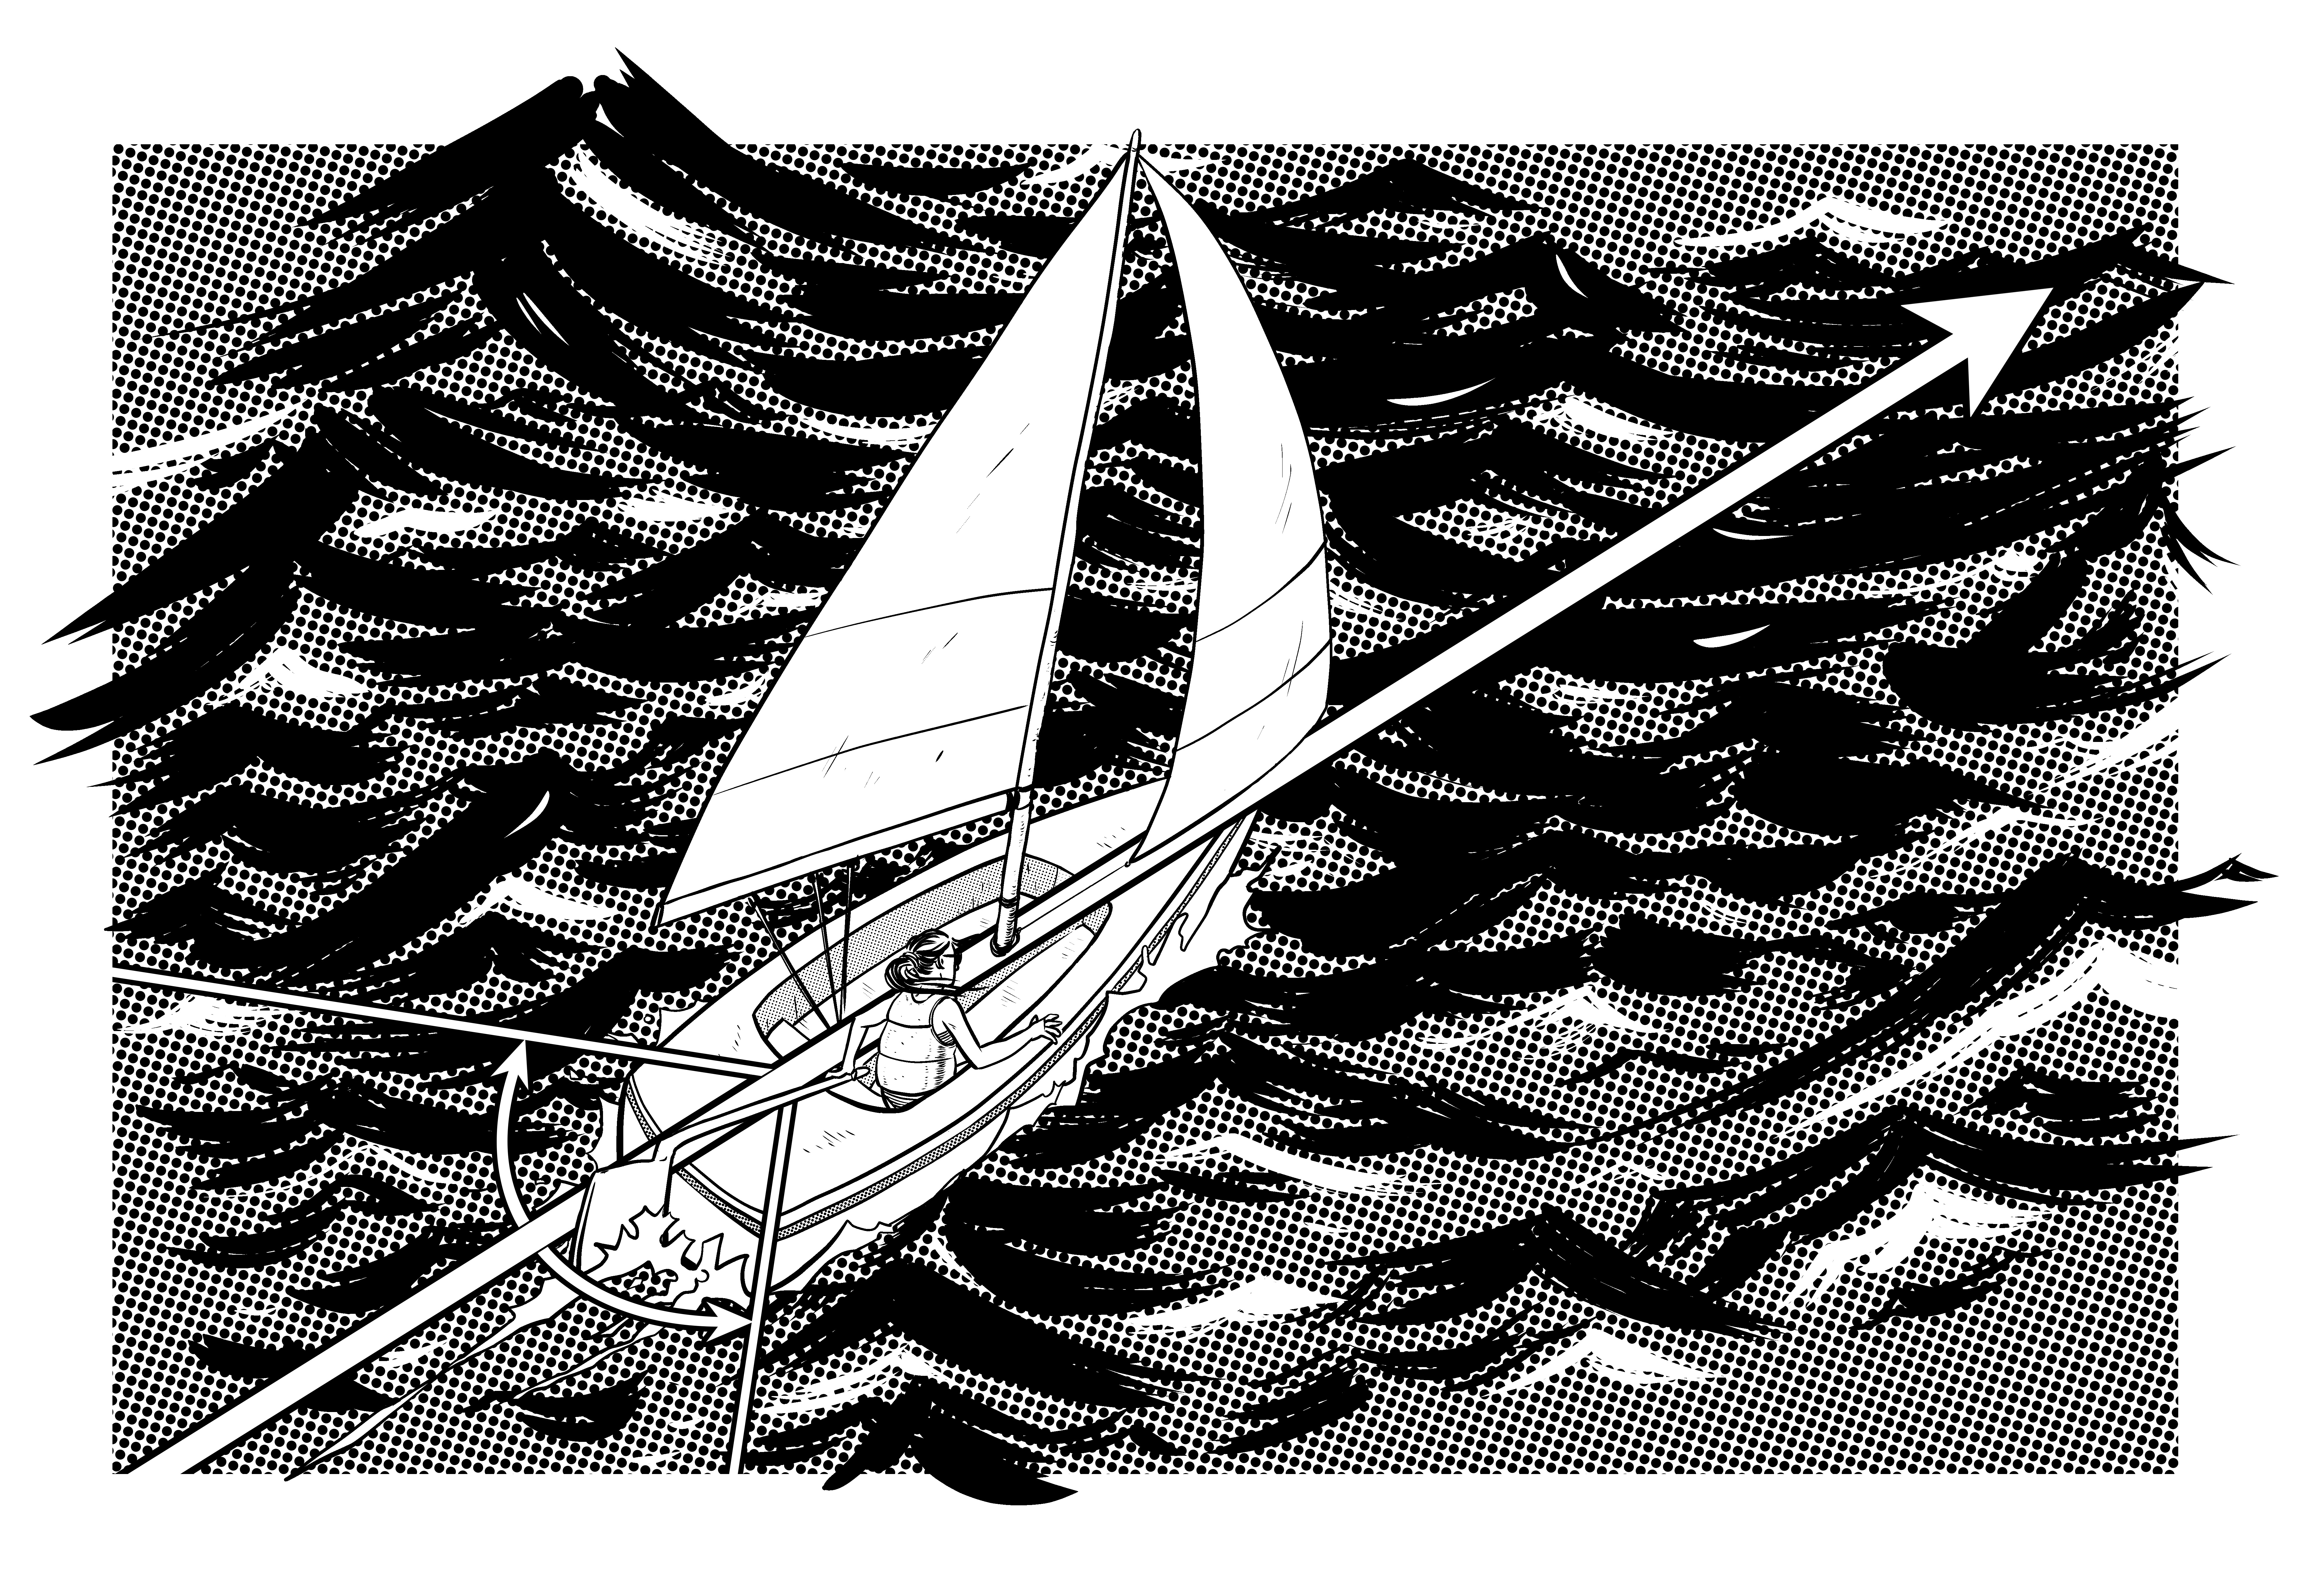
\includegraphics[scale=0.04]{./lecture_includes/scottboat.jpg}
  \end{figure}

\end{frame}

\subsection{Origins of causal inference}


\begin{frame}{Three New Ideas}

\begin{enumerate}
\item \textbf{Counterfactual}: Philosophers come to it first and its central role in causal inference makes causality \emph{unknowable} that the project is nearly derailed
\item \textbf{Treatment assignment mechanism}: Neyman and Fisher solve the counterfactual problem in statistics and lay the foundation of the modern randomized controlled trial (RCT) with their focus on the selection process
\item \textbf{No One Causal Effect}: There is no such thing as ``the causal effect''; there's many and your first step is to pick a parameter (not as easy as it sounds)
\end{enumerate}


\end{frame}



\begin{frame}{Modern Philosophers Introduce Counterfactual Comparisons}

\begin{quote}
    ``If a person eats of a particular dish, and dies in consequence, that is, would not have died if he had not eaten it, people would be apt to say that eating of that dish was the source of his death.'' -- John Stuart Mill (19th century moral philosopher and economist)
\end{quote}

\bigskip
  
    \begin{quote}
    ``Causation is something that makes a difference, and the difference it makes must be a difference from what would have happened without it.'' -- David Lewis (20th century philosopher)
\end{quote}

\end{frame}

  
\begin{frame}{Counterfactuals Almost Derailed Causal Inference}



Mill's counterfactuals were immensely valuable for the clarity of the definition as well as its intuitive validity of causality, but it came at a huge price 

\bigskip

If I have to know what would have happened had I not eaten the dish, but I did eat the dish, then isn't it actually impossible to know the causal effect of eating the dish?

\bigskip

Statisticians surprisingly resolve this tension in the early 20th century with the introduction of notation and the principles of treatment assignment


\end{frame}


\begin{frame}{Statistical origins}

\begin{quote}
``Yet, although the seeds of the idea that [causal effects are comparisons of potential outcomes] can be traced back at least to the 18th century [most likely he means David Hume], the formal notation for potential outcomes was not introduced until 1923 by Neyman.'' -- Don Rubin (1990)
\end{quote}

\end{frame}


\begin{frame}{Jerzy Neyman's Notation}

\begin{itemize}
\item Jerzy Neyman's 1923 article describes a field experiment with differing plots of land (imagine hundreds of square gardens) and many different ``varieties'' of fertilizer that farmers could apply to the land
\item ``$U_{ik}$ is the yield of the $i$th variety on the $k$th plot...'' (Neyman 1923)
\item He calls $U_{ik}$ ``potential yield'', as opposed to the realized yield because $i$ (the fertilizer type) described all possible fertilizers that could be assigned to each $k$ square garden
\item Though only one fertilizer will be assigned to the land, many possible fertilizer assignments were possible beforehand, each with their own outcome
\end{itemize}

\end{frame}

\begin{frame}{Jerzy Neyman's Notation}

\begin{itemize}

\item For each fertilizer there is an associated ``potential yield'' that he collapses into $U$ which he considers to be ``a priori fixed but unknown'' (Rubin 1990)
\item Farmers draw fertilizer from an urn, like a bingo ball from a bingo ball machine, with replacement and apply it to each square garden
\item Fertilizer assignment moves us from ``all possible outcomes'' to ``realized outcome'' terminology
\item Neyman's urn model was a classic thought experiment, but it was also stochastically identical to the completely randomized experiment
\item His arch-rival, Ronald Fisher, realizes this and publishes a book two years later calling for \emph{randomizization} as the basis for causal inference
\end{itemize}

\end{frame}

\begin{frame}{Treatment assignment mechanism}

\begin{quote}

``Before the 20th century, there appears to have been only limited awareness of the concept of the assignment mechanism.  Although by the 1930s, randomized experiments were firmly established in some areas of scientific investigation, notably in agricultural experiments, there was no formal statement for a general assignment mechanism and, moreover, not even formal arguments in favor of randomization until Fisher (1925).'' (Imbens and Rubin 2015)

\end{quote}

\end{frame}

\begin{frame}{Progress is made and progress is not made}

\begin{itemize}

\item Econometrics traditionally modeled causality in terms of realized outcomes until recently (with some exceptions)
\item We need to make a distinction between now the idea of data (``realized outcomes'') and these hypothetical concepts represented by Neyman's notation (``potential outcomes'')

\end{itemize}


\end{frame}

\subsection{Treatment Effects}

\begin{frame}{Potential outcomes notation}

Let the treatment be a binary variable: $$D_{i,t} =\begin{cases} 1 \text{ if placed on ventilator at time $t$} \\ 0 \text{ if not placed on ventilator at time $t$} \end{cases}$$where $i$ indexes an individual observation, such as a person
\end{frame}

\begin{frame}{Potential outcomes notation}

Potential outcomes: $$Y_{i,t}^j =\begin{cases} 1 \text{ health if placed on ventilator at time $t$} \\ 0 \text{ health if not placed on ventilator at time $t$} \end{cases}$$where $j$ indexes a potential treatment status for the same $i$ person at the same $t$ point in time
\end{frame}


\begin{frame}{Realized vs potential outcomes}

  \begin{itemize}
    \item Potential outcome $Y^1$ refers to the ``a priori fixed but unknown'' outcomes associated with different possible treatment assignments
    \item Realized outcome $Y$ refers to the ``posterior and known'' outcome associated with a specific treatment assignment
    \item Potential outcomes become realized outcomes through treatment assignment generated by an assignment mechanism like randomization or rationality
  \end{itemize}
\end{frame}


\begin{frame}{Models vs Treatment Assignment}

\begin{itemize}
    \item Treatment assignment \emph{mechanism} drives the entire effort to identify causal effects as some make it easy and some make it potentially \emph{impossible}
	\item Put another way, the same model can be unbiased and biased depending on the treatment assignment and be utterly detectable otherwise
	\item Means modeling does not come first -- it comes last
	\end{itemize}
\end{frame}

\begin{frame}{Important definitions}

    \begin{block}{Definition 1: Individual treatment effect}
      The individual treatment effect,  $\delta_i$, associated with a ventilator is equal to $Y_i^1-Y_i^0$.
    \end{block}
\end{frame}


\begin{frame}{Important definitions}


    \begin{block}{Definition 2: Switching equation}
      An individual's realized health outcome, $Y_i$, is determined by treatment assignment, $D_i$ which selects one of the potential outcomes:
      \begin{eqnarray*}
        Y_i& = D_iY^1_i+(1-D_i)Y^0_i& \\
        Y_i& = \begin{cases}
          Y^1_i\text{ if }D_i=1 \\
          Y^0_i\text{ if }D_i=0
        \end{cases}
      \end{eqnarray*}
    \end{block}
    
    Not the same as treatment assignment mechanism.  Treatment assignment mechanism describes how $D$ was assigned, not whether it was assigned.

\end{frame}


\begin{frame}{Missing data problem}


    \begin{block}{Definition 3: Fundamental problem of causal inference}
      If you need both potential outcomes to know causality with certainty, then since it is impossible to observe both $Y_i^1$ and $Y_i^0$ for the same individual, $\delta_i$, is \emph{unknowable}.
    \end{block}

This is my reason from saying Mill's counterfactual framework derailed the quest for causal effects given counterfactuals are fictional
    
\end{frame}




\begin{frame}{Average Treatment Effects}

  \begin{block}{Definition 4: Average treatment effect (ATE)}
    The average treatment effect is the population average of all $i$ individual treatment effects
    \begin{eqnarray*}
      E[\delta_i]&=&E[Y_i^1-Y_i^0]\\
      &=&E[Y^1_i] - E[Y^0_i]
    \end{eqnarray*}
  \end{block}

  \bigskip

Aggregate parameters based on individual treatment effects are \emph{summaries} of individual treatment effects

\bigskip

  Cannot be calculated because $Y^1_i$ and $Y^0_i$ do not exist \emph{for the same unit i} due to switching equation

\end{frame}



\begin{frame}{Conditional Average Treatment Effects}


  \begin{block}{Definition 5: Average Treatment Effect on the Treated (ATT)}
    The average treatment effect on the treatment group is equal to the average treatment effect conditional on being a treatment group member:
    \begin{eqnarray*}
      E[\delta|D=1]&=&E[Y^1-Y^0|D=1] \nonumber \\
      &=&E[Y^1|D=1]-E[Y^0|D=1]
    \end{eqnarray*}
  \end{block}
  Cannot be calculated because $Y^1_i$ and $Y^0_i$ do not exist \emph{for the same unit i} due to switching equation. 


\end{frame}




\begin{frame}{Average Treatment Effects are Simple Summaries}

  \begin{itemize}
	\item Notice how in all three of these, all we did was take the defined treatment effect at the individual and aggregate
	\item Because aggregate causal parameters are \emph{summaries} of individual treatment effects, each of which cannot be calculated, the aggregates cannot be calculated either
	\item Missing data in this context isn't missing your car keys -- it's missing unicorns and fire breathing dragons (fictional vs real data)
	\item While we cannot measure average causal effects, we can estimate them, but only in situations and we review one -- randomization
  \end{itemize}

\end{frame}







\begin{frame}{Simple Comparisons}


  \begin{block}{Definition 7: Simple difference in mean outcomes (SDO)}
    A simple difference in mean outcomes (SDO) can be approximated by comparing the sample average outcome for the treatment group ($D=1$) with a comparison group ($D=0$)
    
    \begin{eqnarray*}
      SDO &=& E[Y^1 | D=1] - E[Y^0 | D=0]
    \end{eqnarray*}
  \end{block}
  \bigskip

SDO is not a causal parameter because it's comparing $Y^1$ and $Y^0$ for different units, not the same units, so what is it measuring? 

\end{frame}


\begin{frame}{Decomposition of the SDO}

  \begin{block}{Decomposition of the SDO}
    The SDO is made up of three things:
    \begin{eqnarray*}
      E[Y^1 | D=1] - E[Y^0 | D=0]&=& ATE\nonumber \\
      &&+ E[Y^0|D=1] - E[Y^0|D=0] \nonumber \\
      && + (1-\pi)(ATT - ATU)
    \end{eqnarray*}
  \end{block}

\bigskip

where $\pi$ is the share of units in the treatment group
\end{frame}


\begin{frame}[plain]

  \begin{block}{Estimate SDO with sample averages}
    \begin{eqnarray*}
      \underbrace{E_N[Y_i | D_i=1] - E_N[Y_i | D_i=0]}_{ \mathclap{\text{Estimate of SDO}}}&=& \underbrace{E[Y^1] - E[Y^0]}_{ \mathclap{\text{Average Treatment Effect}}} \\
      &&+ \underbrace{\alert{E[Y^0|D=1]} - E[Y^0 | D=0]}_{ \mathclap{\text{Selection bias}}}  \\
      && + \underbrace{(1-\pi)(ATT - ATU)}_{ \mathclap{\text{Heterogenous treatment effect bias}}}
    \end{eqnarray*}
  \end{block}

\bigskip

Using the switching equation and sample averages, we can calculate $E_N[Y|D=1] \to E[Y^1 | D=1]$, $E_N[Y|D=0] \to E[Y^0|D=0]$ and $(1-\pi)$ is the share of the population in the control group.

\end{frame}


\begin{frame}{Selection bias}

\begin{itemize}
\item Selection bias in the potential outcomes framework is  two mean potential outcomes differing for two groups,
\item But one of them is fictional and the other isn't
\item Source of the bias is the treatment assignment mechanism
covariates

\end{itemize}

\end{frame}

\begin{frame}{Bias \#1: Selection bias}

  \begin{itemize}
    \item Look very closely at the selection bias terms on their left and right hand sides $$\alert{E[Y^0|D=1]} \neq E[Y^0 |D=0]$$
    \item Most likely, doctors ``selected'' units into and out of treatment based on $Y^0$
    \item Selection bias is caused by a treatment assignment mechanism that selects units into treatment based on $Y^0$ (also called ``sorting'')
    \item We need methods that can "delete" selection bias when making simple comparisons, but the solution isn't statistics -- the solution is to use treatment assignment mechanisms with statistics
      \end{itemize}

\end{frame}

\subsection{Treatment Assignment Mechanisms}


\begin{frame}{What is a Treatment Assignment Mechanism?}
\begin{itemize}
\item Phrase used by Don Rubin and Guido Imbens in their 2015 book referring to concepts dating back to the origins of the randomized experiment methodology in the early 20th century
\item Treatment assignment mechanism refers to the \emph{behavioral reason} that individuals were exposed to some intervention like a poverty program
\item Treatment assignment mechanisms encompasses the entire spectrum of how individuals end up in a particular group or treatment -- randomization is one but not the only one
\end{itemize}
\end{frame}

\begin{frame}{Spectrum of Treatment Assignment}
\begin{itemize}
\item \textbf{Self-selection:} Individuals voluntarily choose based on rationality, desperation, or a desire for improvement.
\begin{itemize}
\item Humans naturally gravitate towards decisions that minimize pain and maximize pleasure.
\item Challenging for causal inference due to selection bias and heterogenous responses to treatments.
\end{itemize}
\item \textbf{Randomization:} Individuals are assigned purely by chance.
\begin{itemize}
\item Contrary to typical human decision-making processes.
\item Simplifies causal inference due to the absence of selection bias.
\end{itemize}
\item Most real-world situations lie between these two extremes.
\item The art of causal inference outside laboratory settings often grapples with these "non-experimental" situations.
\end{itemize}
\end{frame}


\begin{frame}{Treatment Assignment Mechanisms}
\begin{itemize}
\item Ways in which individuals are allocated to a particular treatment or program.
\item Crucial for understanding and isolating the causal effects of the treatment.
\item Five commonly used mechanisms:
\end{itemize}
\end{frame}

\begin{frame}{1) Randomization}
\begin{itemize}
\item Easiest and most straightforward method.
\item Reliably balances determinants of the outcome across groups.
\item Eliminates selection bias and isolates the average treatment effect.
\item Sometimes may not be feasible or ethical, and stakeholders may be opposed to doing it 
\end{itemize}
\end{frame}

\begin{frame}{2) Covariates}
\begin{itemize}
\item People are assumed to be sorting into programs based on observable characteristics, but for people with identical characteristics, the sorting is random
\item Methods like propensity scores or matching.
\item Behavior is complex, often challenging to capture solely with covariates.
\end{itemize}
\end{frame}


\begin{frame}{3) Instrumental Variables (IV)}
\begin{itemize}
\item People get into a program, not because they're in an experiment, and not because of their observable characteristics, but because of a random event called the instrumental variable
\item Requires that the researcher know of and have proper measurements of a naturally occurring randomization.
\item Example: Regions randomly assign defendants to courts who have different judges with different tendencies to convict; this allows us to estimate the effect of conviction on life outcomes -- an RCT we could never run
\end{itemize}
\end{frame}



\begin{frame}{4) Running Variables}
\begin{itemize}
\item People take a test, and if their score on the test exceeds some number, administrators put them into the social program
\item It isn't random, but depending on the nature of the effort put into the test, can still be used to estimate the effect of the social program on life outcomes
\item Example: Being assigned to a welfare program based on fixed income
\end{itemize}
\end{frame}

\begin{frame}{Takaful and Karama Program}
\begin{itemize}
\item Initiated in 2015 as part of Egypt's economic reforms from 2014.
\item Targeted cash transfers to poor households.
\item Two main assignment mechanisms used: IV and Running Variables.
\end{itemize}
\end{frame}

\begin{frame}{Focus of our Discussion}
\begin{itemize}
\item We will delve deeper into Instrumental Variables (IV) and Running Variables.
\item These mechanisms, combining randomized experiments and non-randomized scoring, are pivotal in the evaluation of Takaful and Karama.
\end{itemize}
\end{frame}



\section{Takaful and Karama Impact Evaluation}

\subsection{Description of program and methodology}

% Slide 1
\begin{frame}{Takaful and Karama Programs}
\begin{itemize}
    \item \textbf{Takaful (Solidarity):} A \textit{conditional} cash transfer program targeting poor families with children under 18 years of age. Conditions for school attendance and health care utilization were planned but not yet implemented.
    \item \textbf{Karama (Dignity):} An \textit{unconditional} cash transfer program targeting the elderly (aged 65 and above) and persons with severe disabilities.
\item Initiated in 2015, part of Egypt's economic reforms since 2014, co-financed by the Egyptian government and the World Bank.
\end{itemize}
\end{frame}

% Slide for Europe
\begin{frame}{Poverty Rate Comparison: Europe (2015)}

Egypt poverty in context

\begin{itemize}
    \item \textbf{Egypt}: Poverty rate in 2015: 27.8\%.
    \item \textbf{United Kingdom}: Approx. 15\% (below 60% of median income)
    \item \textbf{Germany}: 16.7\%
    \item \textbf{France}: 14\%
\end{itemize}
\small Note: Comparisons can vary due to different poverty measurement methods.
\end{frame}

% Slide for North America
\begin{frame}{Poverty Rate Comparison: North America (2015)}
Egypt poverty in context

\begin{itemize}
    \item \textbf{Egypt}: Poverty rate in 2015: 27.8\%.
    \item \textbf{United States}: 13.5\%
    \item \textbf{Canada}: 9.5\% (Low Income Measure, After Tax)
\end{itemize}
\small Note: Comparisons can vary due to different poverty measurement methods.
\end{frame}

% Slide for Middle East
\begin{frame}{Poverty Rate Comparison: Middle East (Around 2015)}
Egypt poverty in context

\begin{itemize}
    \item \textbf{Egypt}: Poverty rate in 2015: 27.8\%.
    \item \textbf{Yemen} (Upper bound): >50\% (before conflict intensification)
    \item \textbf{Jordan} (Lower bound): 14.4\% (2010 estimate, might have changed after Syrian refugee crisis)
\end{itemize}
\small Note: Comparisons can vary due to different poverty measurement methods.
\end{frame}





% Slide 3
\begin{frame}{Egyptian Context, Survey and Data Collection}
\begin{itemize}
\item Post-economic reforms: Likely increase in poverty due to rising price levels.
\item Study's consumption survey: 40\% below the 2015 poverty line (EGP 482 per capita/month).
\item Survey conducted from July 15 – August 30, 2017.
\item Data on expenditure, well-being, schooling, health, nutrition, decision-making, shocks.
\item Total sample: 6,541 households for evaluation + 1,692 for targeting analysis.
\end{itemize}
\end{frame}

% Slide 4
\begin{frame}{RDD and IV}
\begin{itemize}
\item People are assigned into cash transfer programs, not so much because they volunteered, but because their ``score'' on some ``test'' passed some ``cutoff'' of eligibility
\item Insofar as people are voluntarily sorting into the program, and thus bypassing the threshold eligibility rule, then selection bias gets reintroduced
\item Authors will augment the RD approach with the instrument approach
\end{itemize}
\end{frame}

% Slide 4
\begin{frame}{PMT Score and Eligibility Rule}
\begin{itemize}
\item Households selected based on Proxy Means Test (PMT) score across three waves.
\item Compares outcomes for beneficiaries below vs. non-beneficiaries above the threshold.
\item Large number of households with PMT score near eligibility thresholds.
\end{itemize}
\end{frame}


% Slide 5
\begin{frame}{PMT Score and Eligibility}
\begin{itemize}
\item Three thresholds of PMT score determine eligibility.
\item Covariate based methods (e.g., propensity scores) ruled out due to lack of pre-program baseline data.
\item Used two methods for impact estimation: IV and Fuzzy RD.
\end{itemize}
\end{frame}

% Slide explaining PMT and its role in Takaful and Karama Programs
\begin{frame}{Proxy Means Test (PMT) and Program Enrollment}
\begin{itemize}
    \item \textbf{Proxy Means Test (PMT):} A tool used to estimate household's economic well-being based on observable household attributes. 
    \item \textbf{PMT Score Generation:} Derived from data collected during three waves of registration. Households are given scores based on various socio-economic indicators.
    \item \textbf{Eligibility Rule:} Households with PMT scores below a set threshold become eligible for the programs.
\end{itemize}
\end{frame}



\subsection{Takaful Impact}

% Slide for Introduction to Takaful Results
\begin{frame}{Takaful Impact Results: Introduction}
\begin{itemize}
    \item Takaful aimed to assist poor households by increasing household consumption.
    \item Impact comparable to successful cash transfer programs in other countries.
    \item Significant reduction in the prevalence of poverty among beneficiaries.
\end{itemize}
\end{frame}

% Slide for Food Consumption & Diet Quality
\begin{frame}{Takaful Impact Results: Food Consumption \& Diet Quality}
\begin{itemize}
    \item Beneficiaries increased food consumption by 8.3 - 8.9\% per AEU.
    \item Notable increase in value of fruit and meat consumption.
    \item No significant impact on dietary diversity, possibly due to already diverse diets.
\end{itemize}
\end{frame}

% Slide for Child Nutrition
\begin{frame}{Takaful Impact Results: Child Nutrition}
\begin{itemize}
    \item Positive impact on weight-for-height z-scores for children under 2.
    \item Reduction in children under 5 treated for malnourishment.
    \item No significant change in rates of child stunting.
\end{itemize}
\end{frame}

% Slide for Women’s Decision Making
\begin{frame}{Takaful Impact Results: Women’s Decision Making}
\begin{itemize}
    \item 90\% of Takaful beneficiaries were female as of June 2017.
    \item Negative impact on women’s control over decision making.
    \item Contrary to patterns found in other countries and intended program impact.
\end{itemize}
\end{frame}

\begin{frame}{Exploring Takaful's Impact on Women’s Decision Making}
\begin{itemize}
    \item \textbf{Unexpected Finding:} Takaful's negative impact on women’s decision-making is counterintuitive.
    \item \textbf{Potential Selection Bias:} Women with already limited decision-making power may have been more likely to enroll.
    \item \textbf{Absence of Baseline Data:} Without initial data, hard to determine if the program caused the observed outcome.
    \item \textbf{Cultural Dynamics:} External financial support might alter household power dynamics, potentially leading to conflicts.
    \item \textbf{Next Steps:} Qualitative studies can offer deeper insights into household dynamics and perceptions.
\end{itemize}
\end{frame}


% Slide for Schooling and Healthcare
\begin{frame}{Takaful Impact Results: Schooling and Healthcare}
\begin{itemize}
    \item No significant impacts on school enrollment or health care utilization.
    \item Increased spending on school supplies and transportation.
    \item Likely due to absence of conditionalities at evaluation time.
\end{itemize}
\end{frame}


\subsection{Karama Impact}

% Slide for Introduction to Karama Results
\begin{frame}{Karama Impact Results: Introduction}
\begin{itemize}
    \item The RD approach faced challenges due to a shifting inclusion threshold.
    \item More than half of the intended Karama comparison group was lost.
\end{itemize}
\end{frame}

% Slide for Karama's Sample and Challenges
\begin{frame}{Karama Impact Results: Challenges}
\begin{itemize}
    \item Smaller sample size due to the program's smaller scale.
    \item Efficiency in enrolling newly eligible households led to a loss of comparison group.
\end{itemize}
\end{frame}

% Slide for Lack of Measured Impact
\begin{frame}{Karama Impact Results: Measured Impact}
\begin{itemize}
    \item No measurable impacts on outcome variables examined.
    \item Karama transfers represented 28\% of household expenditure per person.
    \item Lack of impact likely due to challenges faced in the study.
\end{itemize}
\end{frame}


\end{document}

\begin{frame}{Randomization}


  \begin{block}{Independence assumption}
    Treatment is assigned to a population independent of that population's potential outcomes  $$(Y^0,Y^1)\independent{D}$$
  \end{block}
  This is random or quasi-random assignment and ensures mean potential outcomes for the treatment group and control group are the same.  Also ensures other variables are distributed the same for a large sample.
  \begin{eqnarray*}
    \alert{E[Y^0|D=1]} &=& E[Y^0 | D=0] \\
    E[Y^1|D=1] &=& \alert{E[Y^1 | D=0]}
  \end{eqnarray*}
\end{frame}

\begin{frame}{Random Assignment Solves the Selection Problem}

  \begin{eqnarray*}
    \underbrace{E_N[y_i | d_i=1] - E_N[y_i | d_i=0]}_{ \mathclap{\text{SDO}}}&=& \underbrace{E[Y^1] - E[Y^0]}_{ \mathclap{\text{Average Treatment Effect}}} \\
    &&+ \underbrace{E[Y^0|D=1] - E[Y^0 | D=0]}_{ \mathclap{\text{Selection bias}}}  \\
    && + \underbrace{(1-\pi)(ATT - ATU)}_{ \mathclap{\text{Heterogenous treatment effect bias}}}
  \end{eqnarray*}


  \begin{itemize}
    \item If treatment is independent of potential outcomes, then swap out equations and \textbf{selection bias} zeroes out:
          \begin{eqnarray*}
            E[Y^0 | D=1] - E[Y^0 | D=0] &=& 0
          \end{eqnarray*}
  \end{itemize}

\end{frame}

\begin{frame}[shrink=20,plain]
  \begin{center}
    \textbf{Random Assignment Solves the Heterogenous Treatment Effects}
  \end{center}

  \begin{itemize}
    \item How does randomization affect heterogeneity treatment effects bias from the third line?  Rewrite definitions for ATT and ATU:\begin{eqnarray*}
            \text{ATT} = E[Y^1 | D=1] - E[Y^0 | D=1] \\
            \text{ATU} = E[Y^1 | D=0] - E[Y^0 | D=0] \\
          \end{eqnarray*}
    \item Rewrite the third row bias after $1-\pi$:\begin{eqnarray*}
            ATT - ATU &=& \textbf{E[Y$^1$ $|$ D=1]} - E[Y^0 | D=1] \\
            && - \textbf{E[Y$^1$ $|$ D=0]} + E[Y^0 | D=0] \\
            &=& 0
          \end{eqnarray*}
    \item If treatment is independent of potential outcomes, then:\begin{eqnarray*}
            E_N[y_i | d_i=1] - E_N[y_i | d_i=0]  &=& E[Y^1] - E[Y^0] \\
            SDO &=& ATE
          \end{eqnarray*}
  \end{itemize}
\end{frame}



\begin{frame}[plain]

  \begin{block}{Identification with Randomization}
    \begin{eqnarray*}
      \underbrace{E_N[Y_i | D_i=1] - E_N[Y_i | D_i=0]}_{ \mathclap{\text{Estimate of SDO}}}&=& \underbrace{E[Y^1] - E[Y^0]}_{ \mathclap{\text{Average Treatment Effect}}} \\
    &&+ \underbrace{0}_{ \mathclap{\text{Selection bias}}}  \\
    && + \underbrace{0}_{ \mathclap{\text{Heterogenous treatment effect bias}}}
    \end{eqnarray*}
  \end{block}
  
  SDO is unbiased estimate of ATE with randomized treatment assignment because it sets selection bias to zero and $ATT=ATU$.



\end{frame}

